\chapter{Microcontrollers for RAILS}
\section{Introduction}
\gls{rails} is a software model and implementation of an automated system to assist the model railroader achieve realism in the operation of a model railroad.
There are four user interface \gls{spa} that provide different aspects of rails they are:
\begin{itemize}
  \item \gls{rsrm} allows the user to match a rfid tag to a rollingstock's road name and number;
  \item \gls{mrim} allows the user to create, update and delete model railroad assets, such as rolling stock;
  \item \gls{mppm} allows the user to enter information about their projects and purchases; and
  \item \gls{mrlm} allows the user to enter information about their layout and control elements of it.
\end{itemize}
\section{RSRM Components}
The implementation of \gls{rsrm} consists of the following micro-services components:
\begin{itemize}
\item \gls{rfid} Controller is a micro-controller that processes \gls{rfid} tags obtained from a \gls{rfid} reader and then publishes \gls{iot} messages to the \gls{mqtt} Broker;
\item \gls{mqtt} Broker is responsible for receiving \gls{rfid} and micro info messages, filtering them, posting to designated topics and sending messages to clients subscribing to topics. The subscribers and publishers bridge the \gls{mqtt} elements with the GUI applications. The broker handles \gls{iot} messages;
\item \gls{isrs} subscribes to \gls{rfid} messages and pushes them via a web-socket to the rsm component;
\item \gls{isms} that subscribes to micro controller startup and heartbeat messages, updating the micros collection via \gls{rlds};
\item \gls{rlds} provides \gls{rest} access to model railroad layout collections including micros;
\item \gls{rids} provides \gls{rest} access to railroad inventory collections including rollingstock;
\item MongoDB a NoSQL database program that stores data records as documents which are gathered in collections. A database stores one or more collections of documents;
\item \gls{mr} Data is the document repository, used by MongoDB, to store complete collections of items such as rollingstock, industries (producers and consumers), track elements, turnouts, projects, purchases, etc. in support of \gls{rails}; and
\item \gls{rsrm} is the \gls{spa} that allows a user to match a \gls{rfid} tag to a rollingstock's road name and number.
\end{itemize}
Figure \ref{fig:rsms-ms-components} depicts the micro-services used to create the rolling stock \gls{rfid} management subsystem.

\begin{figure}[H]
	\centering
		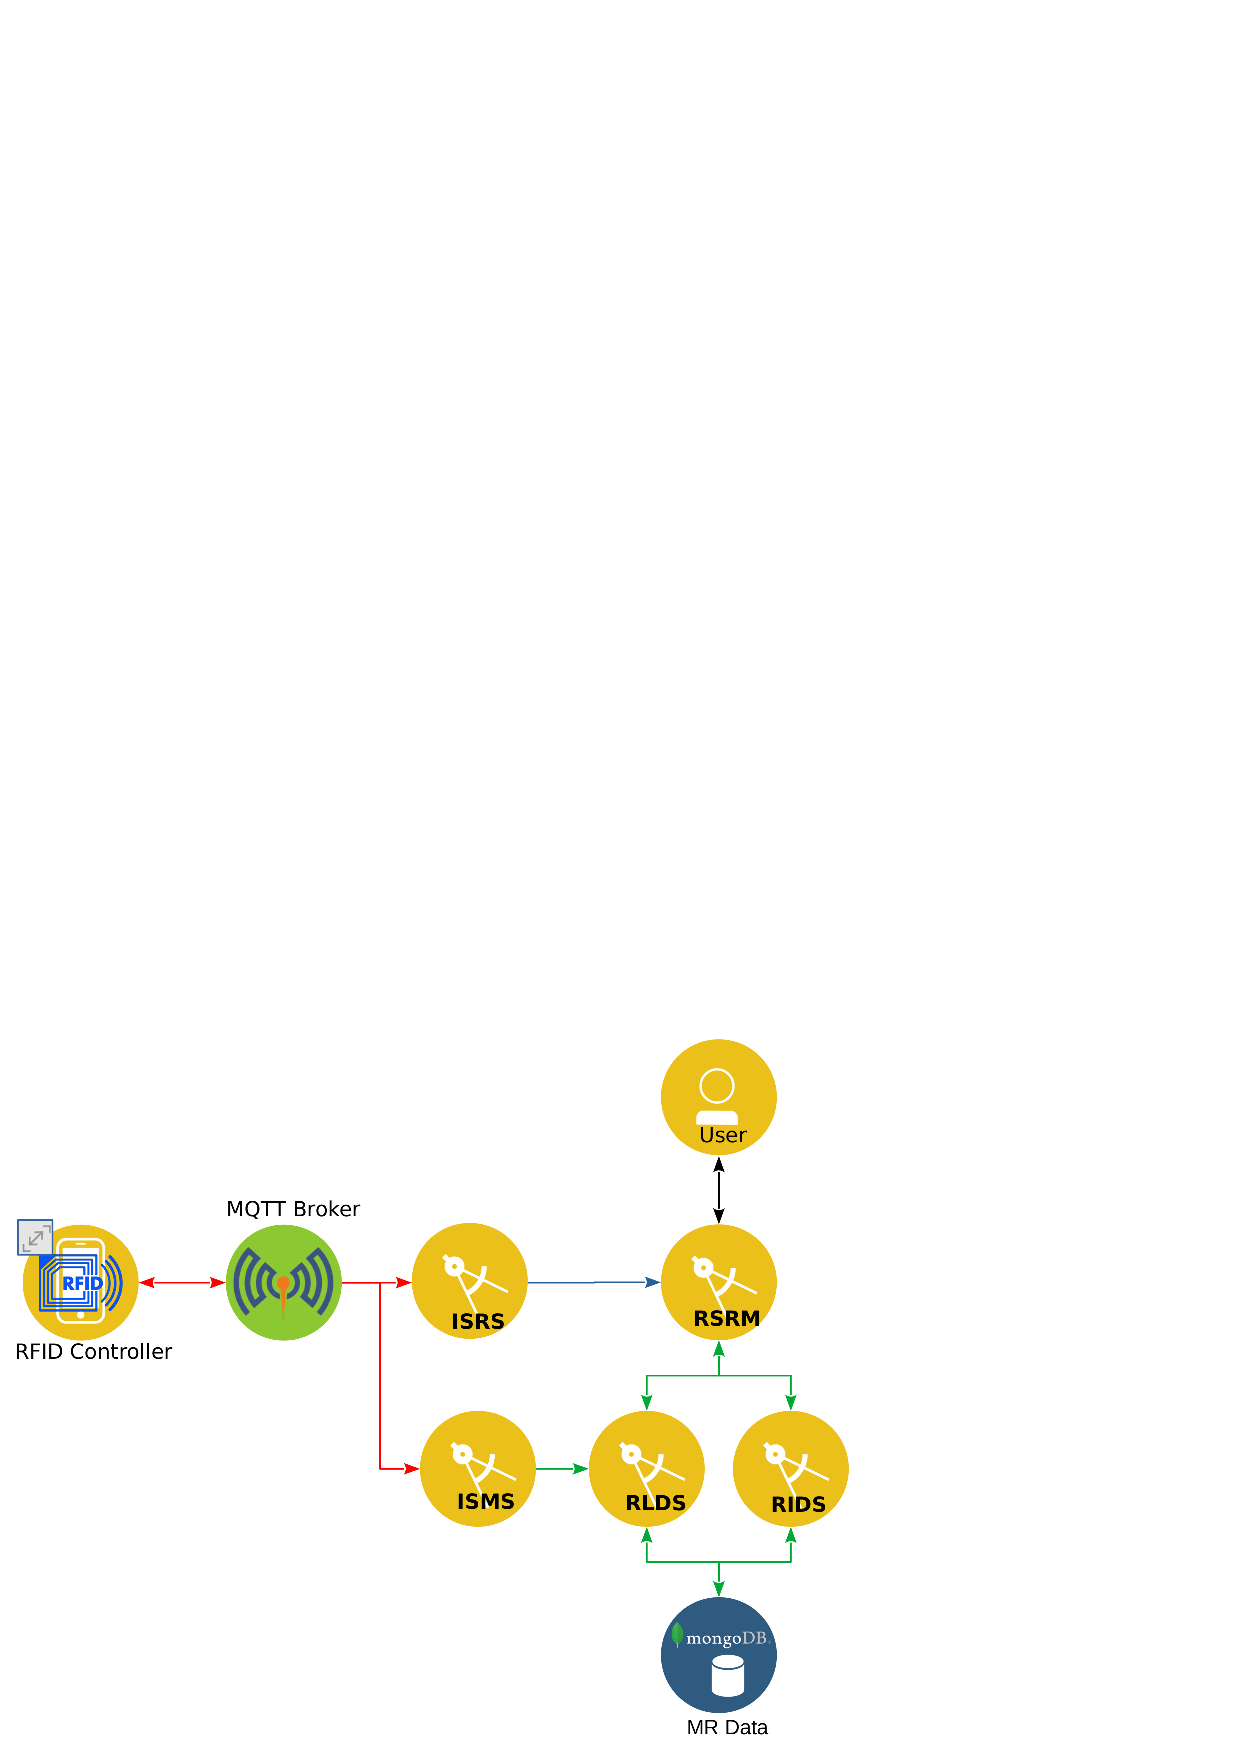
\includegraphics[scale=0.15]{rsms_design.png}
	\caption{Microservices Components}
	\label{fig:rsms-ms-components}
\end{figure}

Three system components that make up this subsystem:
\begin{itemize}
\item \gls{rfid} Controller is a micro-controller that processes \gls{rfid} tags obtained from a \gls{rfid} reader and then publishes \gls{iot} messages to the \gls{mqtt} Broker;
\item Network is a \gls{tcpip} communication medium that connects the \gls{rfid} Controller, \gls{mqtt} Broker and \gls{rsrm} components; and
\item Host is a computer that runs the \gls{mqtt} Broker and other \gls{rsrm} micro-services components.
\end{itemize}
Figure \ref{fig:rsms-system} depicts the systems components used to create the rolling stock \gls{rfid} management subsystem.

\begin{figure}[H]
	\centering
		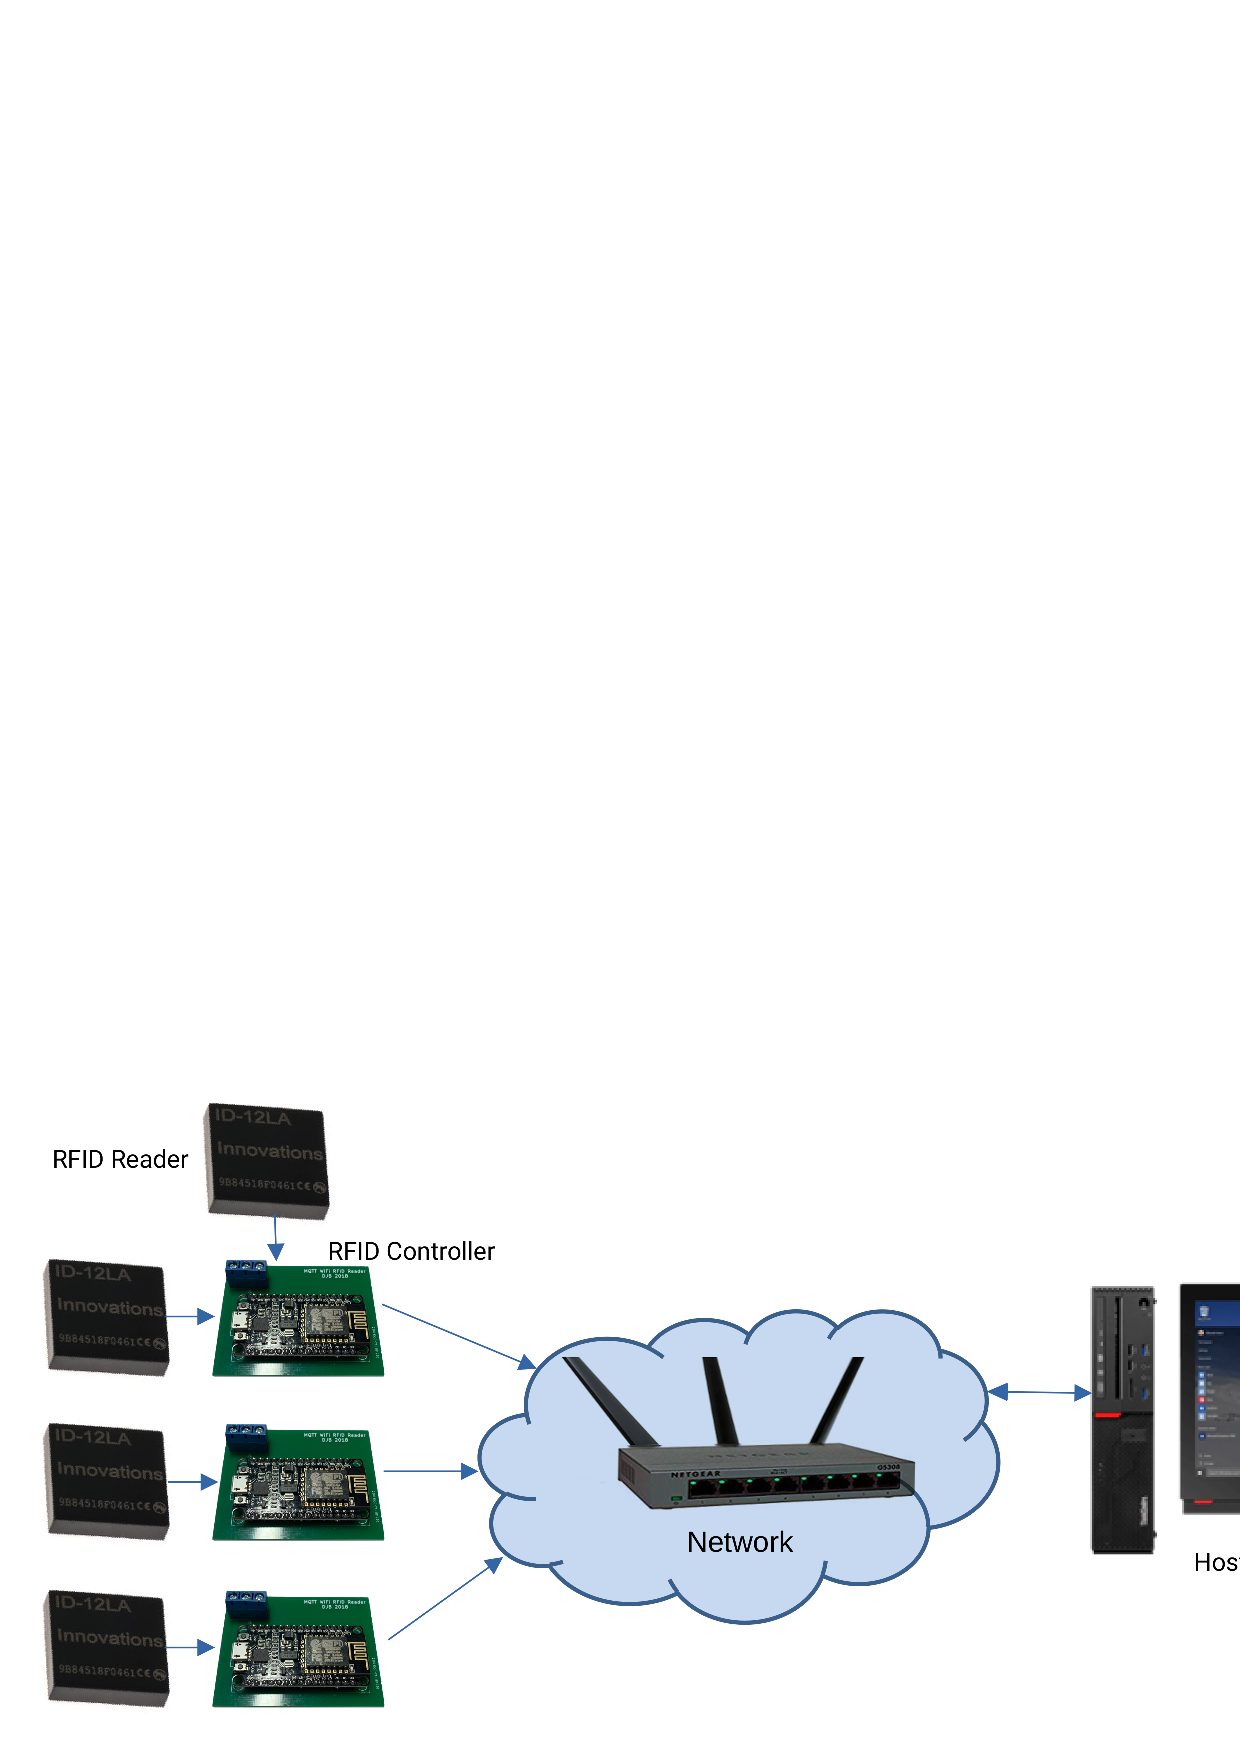
\includegraphics[scale=0.15]{rsms_system.png}
	\caption{MSystem Components}
	\label{fig:rsms-system}
\end{figure}

\section{MRLM System Components}

Figure \ref{fig:mrlm-ms-components} depicts the micro-services used to create the

\begin{figure}[H]
	\centering
		\includegraphics[scale=0.8]{mrlm_design.png}
	\caption{Microservices Components}
	\label{fig:mrlm-ms-components}
\end{figure}


\begin{figure}[H]
	\centering
		\includegraphics[scale=0.2]{turnout_system.png}
	\caption{MSystem Components}
	\label{fig:turnout-system}
\end{figure}